\chapter{Methods}

\section{Distillation Formalism} \label{sec:distillation_formalism}

Following the notation of on-policy generalized knowledge distillation \cite{agarwalOnPolicyDistillationLanguage2024}, let $x$ denote a prompt, let $V$ denote the vocabulary, and let $y = (y_1, y_2, \ldots, y_{L_y})$ denote an output sequence. The prefix before token $y_n$ is $y_{<n} = (y_1, \ldots, y_{n-1})$. We write the student policy as $\pi_\theta(\cdot \mid x, y_{<n})$ and the teacher policy as $\pi_T(\cdot \mid x, y_{<n})$, both of which define next-token distributions over $V$.

The simplest distillation objective treats a target sequence as a hard label and trains the student with cross-entropy. If $\mathcal{D}$ is a dataset of prompt--completion pairs, where the completions can be human-written or sampled from the teacher, the loss is

\begin{equation}
\mathcal{L}_{\mathrm{CE}}(\theta)
= \mathrm{E}_{(x,y) \sim \mathcal{D}}
\left[
- \sum_{n=1}^{L_y}
\log \pi_\theta(y_n \mid x, y_{<n})
\right].
\label{eq:xentropy}
\end{equation}

This objective only uses the observed target token $y_n$ at each position. We refer to this method as supervised fine-tuning (SFT) \cite{zotero-item-425}.

A richer form of distillation uses the full teacher distribution over the vocabulary instead of using the token sampled by the teacher. For a fixed prompt and completion, the token-level forward KL from teacher to student is

\begin{equation}
D_{\mathrm{KL}}(\pi_T \| \pi_\theta)(y \mid x)
= \sum_{n=1}^{L_y} \sum_{v \in V}
\pi_T(v \mid x, y_{<n})
\log
\frac{\pi_T(v \mid x, y_{<n})}
{\pi_\theta(v \mid x, y_{<n})}.
\label{eq:forward_kl}
\end{equation}

The reverse KL swaps the order of the two distributions:

\begin{equation}
D_{\mathrm{KL}}(\pi_\theta \| \pi_T)(y \mid x)
= \sum_{n=1}^{L_y} \sum_{v \in V}
\pi_\theta(v \mid x, y_{<n})
\log
\frac{\pi_\theta(v \mid x, y_{<n})}
{\pi_T(v \mid x, y_{<n})}.
\label{eq:reverse_kl}
\end{equation}

The distinction is important because KL divergence is asymmetric. Forward KL averages the log-ratio under the teacher distribution, so it penalizes the student for failing to place probability mass on tokens the teacher considers likely. This makes it a mass-covering objective. Reverse KL averages under the student distribution, so it penalizes tokens the student samples when the teacher assigns them low probability. This makes it more mode-seeking and can be useful when a lower-capacity student cannot match the full teacher distribution.

We show the distinction graphically in Figure~\ref{fig:toy_forward_vs_reverse} using a plot from \cite{guMiniLLMOnPolicyDistillation2026} that shows how the forward and reverse KL fit a Gaussian mixture distribution with a single Gaussian distribution. The reverse KL seeks the major mode of the mixture while the forward KL tries to fit all three.

\begin{figure}[h]
    \centering
    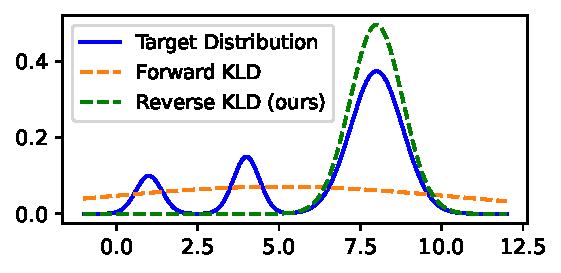
\includegraphics[width=0.5\linewidth]{figures/forward_vs_reverse.pdf}
    \caption{Image from \cite{guMiniLLMOnPolicyDistillation2026} showing the difference of using forward and reverse KL to fit a mixture of three Gaussians. The reverse KL tries to fit the major mode while the forward KL tries to approximate the three modes.}
    \label{fig:toy_forward_vs_reverse}
\end{figure}

On top of the distinction between forward and reverse KL, it is important to distinguish where we sample the rollouts $y$ we use for training. Off-policy distillation samples the rollouts from the teacher policy $y \sim \pi_T(\cdot \mid x)$ and then seeks the feedback from the same teacher. On-policy distillation samples completions from the student and then compares teacher and student distributions on the prefixes that the student actually visits:

\begin{equation}
\mathcal{L}_{\mathrm{OPD}}(\theta)
= 
\mathrm{E}_{y \sim \pi_\theta(\cdot \mid x)}
\left[
D(\pi_T, \pi_\theta)(y \mid x)
\right],
\label{eq:on_policy_distillation}
\end{equation}

where $D$ can be instantiated as the forward KL in Equation~\ref{eq:forward_kl}, the reverse KL in Equation~\ref{eq:reverse_kl}, or another token-level divergence. We can define off-policy distillation analogously by changing $y \sim \pi_\theta(\cdot \mid x)$ for $y \sim \pi_T(\cdot \mid x)$.

In practice, computing the full sums over $V$ can be expensive. A common solution is to The sampled-token reverse-KL formulation used in on-policy distillation keeps only the realized token at each position of a student rollout $\hat{y} \sim \pi_\theta(\cdot \mid x)$. The resulting top-1 sampled-token estimate is

\begin{equation}
\widehat{D}_{\mathrm{KL}}^{\mathrm{top}\mbox{-}1}
(\pi_\theta \| \pi_T)(\hat{y} \mid x)
= \sum_{n=1}^{L_{\hat{y}}}
\left[
\log \pi_\theta(\hat{y}_n \mid x, \hat{y}_{<n})
- \log \pi_T(\hat{y}_n \mid x, \hat{y}_{<n})
\right].
\label{eq:sampled_token_reverse_kl}
\end{equation}

This is the sampled-token analogue of Equation~\ref{eq:reverse_kl}. Rather than matching the full next-token distributions, it scores the token actually produced by the student under both policies.

We can write an analogous formulation for the Equation~\ref{eq:forward_kl}, where we only use the realized token at each position of a teacher rollout $\hat{y} \sim \pi_T(\cdot \mid x)$. Additionally, we use the forward instead of the reverse KL to avoid optimizing a biased surrogate or using importance sampling to correct the off-policy nature of the data.

\begin{equation}
\widehat{D}_{\mathrm{KL}}^{\mathrm{top}\mbox{-}1}
(\pi_T \| \pi_\theta)(\hat{y} \mid x)
= \sum_{n=1}^{L_{\hat{y}}}
\left[
\log \pi_T(\hat{y}_n \mid x, \hat{y}_{<n})
- \log \pi_\theta(\hat{y}_n \mid x, \hat{y}_{<n})
\right].
\label{eq:sampled_token_forward_kl}
\end{equation}

The formulation in Equation~\ref{eq:sampled_token_forward_kl} is equivalent to the soft version of SFT, because we are including the log probability of the token sampled by the teacher instead of excluding it and using it as a hard target as in Equation~\ref{eq:xentropy}.

\section{Top-K KL}


\section{Privileged Context}
